\section{Bài 09}
Xem xét bài toán cực đại
\begin{equation}
    \label{problem:09}
    \begin{aligned}
        \max \quad & x^2 + y\\
        \textrm{s.t.} \quad & x^2 + y^2 \leq 9,\\
        &x + y \leq 1.
    \end{aligned}
\end{equation}
\begin{enumerate}[label=(\alph*)]
    \item Vẽ miền khả thi và đường mức của hàm mục tiêu. Dựa trên đó, đoán cực đại toàn cục.
    \item Lập luận tại sao KKT phải thỏa mãn tại các cực đại toàn cục.
    \item Viết các điều kiện KKT, và sử dụng chúng để xác định tất cả các điểm KKT.
    \item Xác định những điểm KKT thỏa mãn điều kiện cấp hai (cần và đủ).
\end{enumerate}

\begin{solution}

    Các thành phần trong bài toán này như sau:
    \begin{align}
        \begin{aligned}
            f(x,y) &= x^2 + y\\
            g_1(x, y) &= x^2 + y^2 - 9 \\
            g_2(x, y) &= x + y  - 1 \\
        \end{aligned}
    \end{align}
    \begin{enumerate}[label=(\alph*)]
        \item Vẽ miền khả thi và đường mức của hàm mục tiêu. Dựa trên đó, đoán cực đại toàn cục.
        \begin{figure}[h!]
            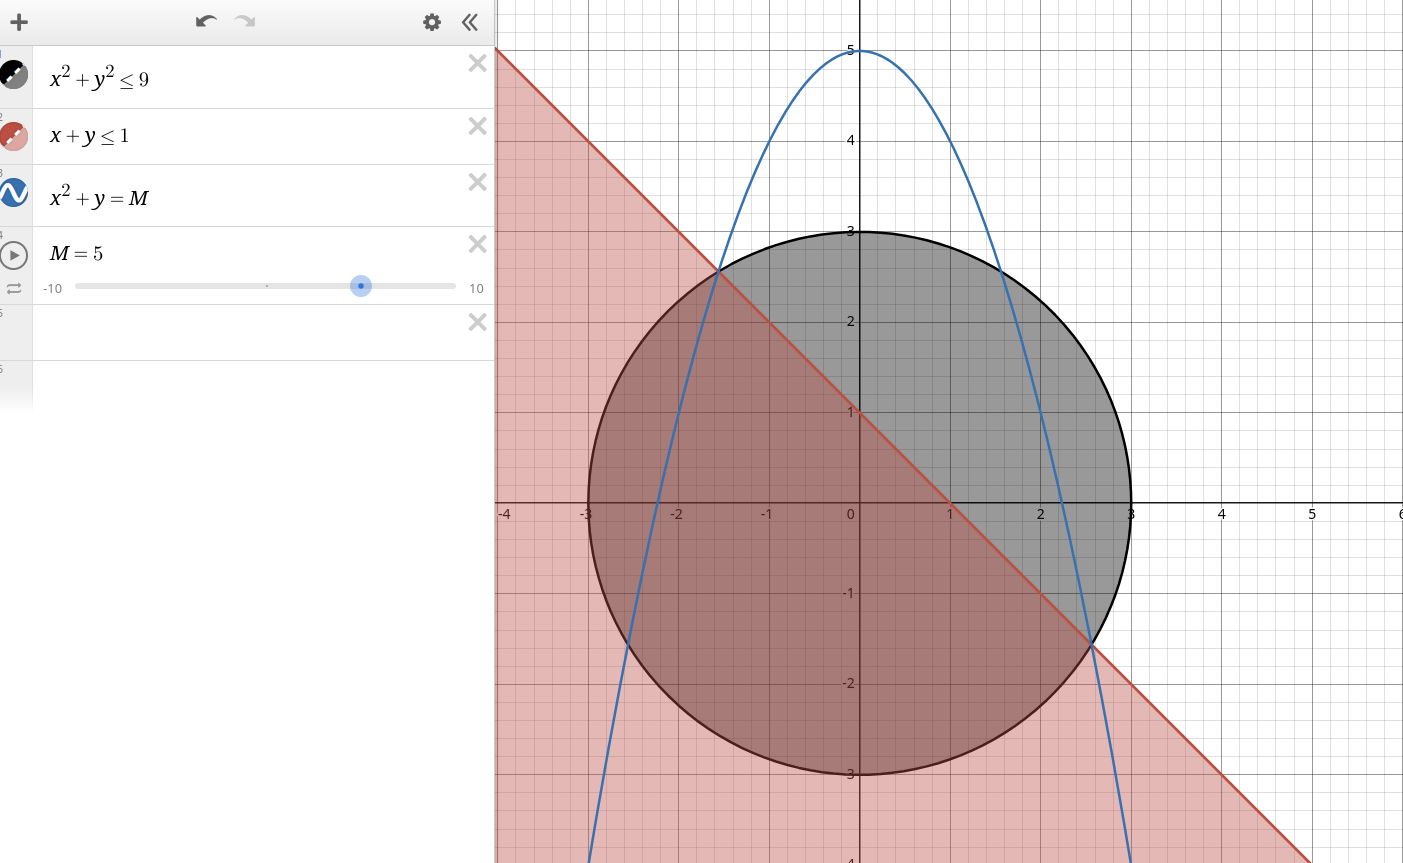
\includegraphics[width=0.85\linewidth]{figures/BT09.png}
            \caption{Miền khả thi của bài toán (\ref{problem:09}).}
            \label{fig:feasible_region_problem_09}
        \end{figure}
        Ta có thể vẽ được miền khả thi và đường múc của hàm mục tiêu như Hình (\ref{fig:feasible_region_problem_09}). Dựa trên hình vẽ, ta có thể đoán được các cực trị của bài toán nằm tại giao điểm giữa các phương trình $f(x,y), g_1(x, y)$ và $g_2(x, y)$. Điểm cực đại sẽ là giao điểm phía trên.
        \item Lập luận tại sao KKT phải thỏa mãn tại các cực đại toàn cục. Ta nhận thấy, bài toán này có cực đại toàn cục bởi vì miền ràng buộc là compact. Ta có đạo hàm của các ràng buộc lần lượt là 
        \begin{itemize}
            \item $\Delta g_1(x, y) = 2(x,y)$ 
            \item $\Delta g_2(x,y) = (1,1)$
        \end{itemize}
        Dễ dàng thấy rằng, đạo hàm thứ hai luôn luôn khác không, và đạo hàm thứ nhất chỉ bằng không tại gốc tọa độ nơi mà không thoả mãn ràng buộc $g1$ không kích hoạt. Do đó, các điều kiện KKT phải được thỏa mãn tại bất kỳ cực tiểu cục bộ $(x^{*}, y^{*})$ nào mà có ít nhất một ràng buộc được kích hoạt. Nếu cả hai ràng buộc được kích hoạt, các đẳng thức $x^{2} + y^{2} = 9$ và $x + y = 1$ cho nghiệm 
        \begin{equation}
            y = \dfrac{1+\sqrt{17}}{2}\quad\text{hoặc}\quad y = \dfrac{1-\sqrt{17}}{2}
        \end{equation}
        và các đạo hàm $\{\Delta g_1(x, y), \Delta g_2(x, y) \}$ độc lập tuyến tính. Do đó, các điều kiện KKT phải thỏa ở ất cả các điểm KKT có thể có.
        \item Viết các điều kiện KKT, và sử dụng chúng để xác định tất cả các điểm KKT. Ta có dạng của hàm Lagrangian như sau:
        \begin{equation}
            L(x,y,\lambda) = x^2 + y + \lambda_1(x^2 + y^2 - 9) + \lambda_2(x + y  - 1)
        \end{equation}
        và các điều kiện KKT được viết như sau:
        \begin{itemize}
            \item \begin{equation}
                \dfrac{\partial L}{\partial x} = 2x + 2\lambda_1x + \lambda_2 = 0 \Leftrightarrow x = -\dfrac{\lambda_2}{2+2\lambda_1}
            \end{equation}
            \item \begin{equation}
                \dfrac{\partial L}{\partial y} = 1 + 2\lambda_1y + \lambda_2 = 0 \Leftrightarrow y = -\dfrac{\lambda_2 + 1}{2\lambda_1}
            \end{equation}
            \item \begin{equation}
                \lambda_1 \geq 0, x^2 + y^2 - 9 \leq 0, \lambda_1(x^2 + y^2 - 9) = 0
            \end{equation}
            \item \begin{equation}
                \lambda_2 \geq 0, x + y  - 1 \leq 0, \lambda_2(x + y  - 1) = 0
            \end{equation}
        \end{itemize}
        Ta xem xét những trường hợp có thể có cho dấu của các nhân tử
        \begin{itemize}
            \item Trường hợp 1 ($\lambda_1 > 0, \lambda_2 > 0)$, ta có hệ
            \begin{equation}
                \begin{cases}
                    x^2 + y^2 - 9 = 0\\
                    x + y  - 1 = 0\\
                \end{cases}
                \Leftrightarrow
                \begin{cases}
                    x = \dfrac{1-\sqrt{17}}{2}\\
                    y = \dfrac{1+\sqrt{17}}{2}
                \end{cases}
                \quad
                \text{hoặc}
                \begin{cases}
                    x = \dfrac{1+\sqrt{17}}{2}\\
                    y = \dfrac{1-\sqrt{17}}{2}
                \end{cases}
            \end{equation}
            Cả hai điểm này đều thỏa mãn ràng buộc nên chúng là các điểm KKT.
            \item Trường hợp 2 ($\lambda_1 = 0, \lambda_2 > 0)$, ta không thể giải được do không xác định cho phương trình (9.6)
            \item Trường hợp 3 ($\lambda_1 > 0, \lambda_2 = 0)$, ta có
            \begin{equation}
                \begin{cases}
                    x = 0\\
                    y = -\frac{1}{2\lambda_1}
                    x^2 + y^2 - 9 = 0\\
                \end{cases}
                \Leftrightarrow
                \begin{cases}
                    x = 0\\
                    \lambda_1 = \pm\dfrac{1}{6}\\
                    y = \pm 3
                \end{cases}
            \end{equation}
            Trong đó $(x, y) = (0, -3)$ thỏa mãn ràng buộc, do đó điểm này là một điểm KKT.
            \item Trường hợp 4 ($\lambda_1 = 0, \lambda_2 = 0)$, ta không thể giải được do không xác định cho phương trình (9.6)
        \end{itemize}
        \item Xác định những điểm KKT thỏa mãn điều kiện cấp hai (cần và đủ).
    \end{enumerate}
\end{solution}